\section{Pyramids and Wavelets}

The \textbf{scale-space} is the family of signals generated by successive smoothing with a Gaussian filter. Using the scale-space we can downsample the image step by step, giving us an \textbf{image pyramid}.
\begin{center}
	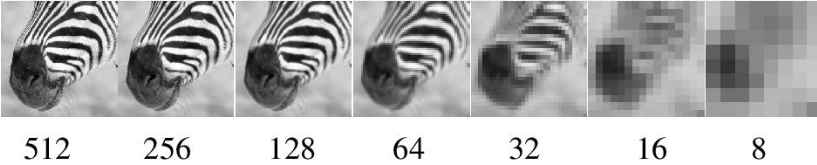
\includegraphics[width=\linewidth]{image_pyramid.png}
\end{center}

Such image pyramids can be used for edge tracking, search for correspondence, etc. One of their main benefits is that they allow for control of detail and computational costs. 


\subsection{The Laplacian Pyramid}

While the Gaussian pyramid successively suppressed high frequencies, the Laplacian pyramid represents a different frequency at each level. This is similar to a bandpass filter.
\begin{center}
	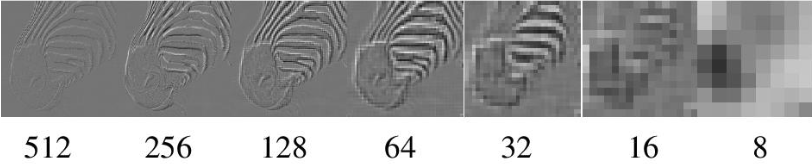
\includegraphics[width=\linewidth]{laplacian_pyramid.png}
\end{center}

With a Laplacian pyramid we mean a difference of Gaussians (DoG). The main benefit is that it removes the redundancy of having the lower frequency parts in every level.


\subsection{Wavelet Transform}

The \textbf{Haar transform} is one of the most basic wavelets.
\begin{center}
	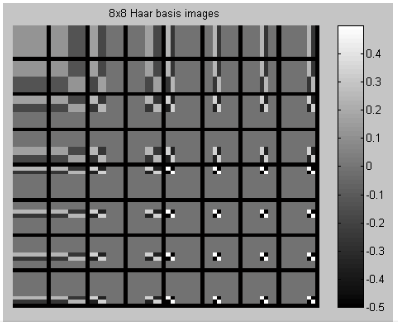
\includegraphics[width=\linewidth]{haar_basis.png}
\end{center}

We can see that the outer vectors correspond to recursively applying a two-band filter to the bands of the previous stage (like a pyramid). The Haar transformation has poor energy compaction, meaning it is not really good for image compression. \medskip

In general wavelet transform works by splitting the signal into a low frequency and a high frequency pass, then the process is applied to the low frequency band recursively.
\begin{center}
	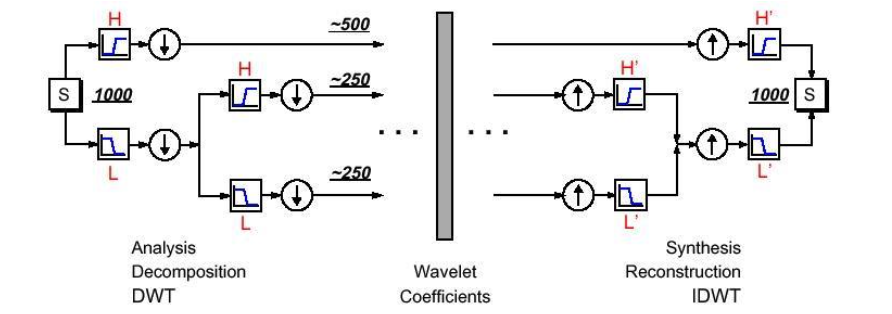
\includegraphics[width=\linewidth]{wavelets.png}
\end{center}

This concept is then again expanded to 2D images.